%%=============================================================================
%% Proof of concept
%%=============================================================================

\chapter{Proof of concept}%
\label{ch:proof-of-concept}

In dit hoofdstuk zal er uitgebreid besproken worden hoe de proof of concept, gebruik makend van SAP Business entity recognition, gebouwd wordt en hoe dit belanghebbende informatie uit een tekst haalt.

\section{Inhoud van de proof of concept}
De proof of concept die in dit onderzoek is gemaakt, bestaat uit een API in python die de Business Entity Recognition service van SAP aanroept en de resultaten teruggeeft. Verder bestaat de proof of concept ook uit een frontend applicatie die de API aanroept en de resultaten weergeeft. De frontend applicatie is een webapplicatie die gebruik maakt van SAP Fiori om een mooie en gebruiksvriendelijke interface te maken.
Tijdens het maken van de proof of concept is er rekening gehouden met de verschillende functionaliteiten die de applicatie zeker moet hebben. Deze functionaliteiten zijn de volgende:
\begin{itemize}
    \item Het uploaden van een service key bestand om een eigen instantie van de Business Entity Recognition service te gebruiken.
    \item Het uploaden van een tekstbestand die de service zal inlezen.
    \item Het kiezen van een bestaand model om de context van de tekst te bepalen en zo betere resultaten te verkrijgen.
    \item De mogelijkheid om de resultaten te bekijken.
\end{itemize}

\begin{figure}[H]
    \centering
    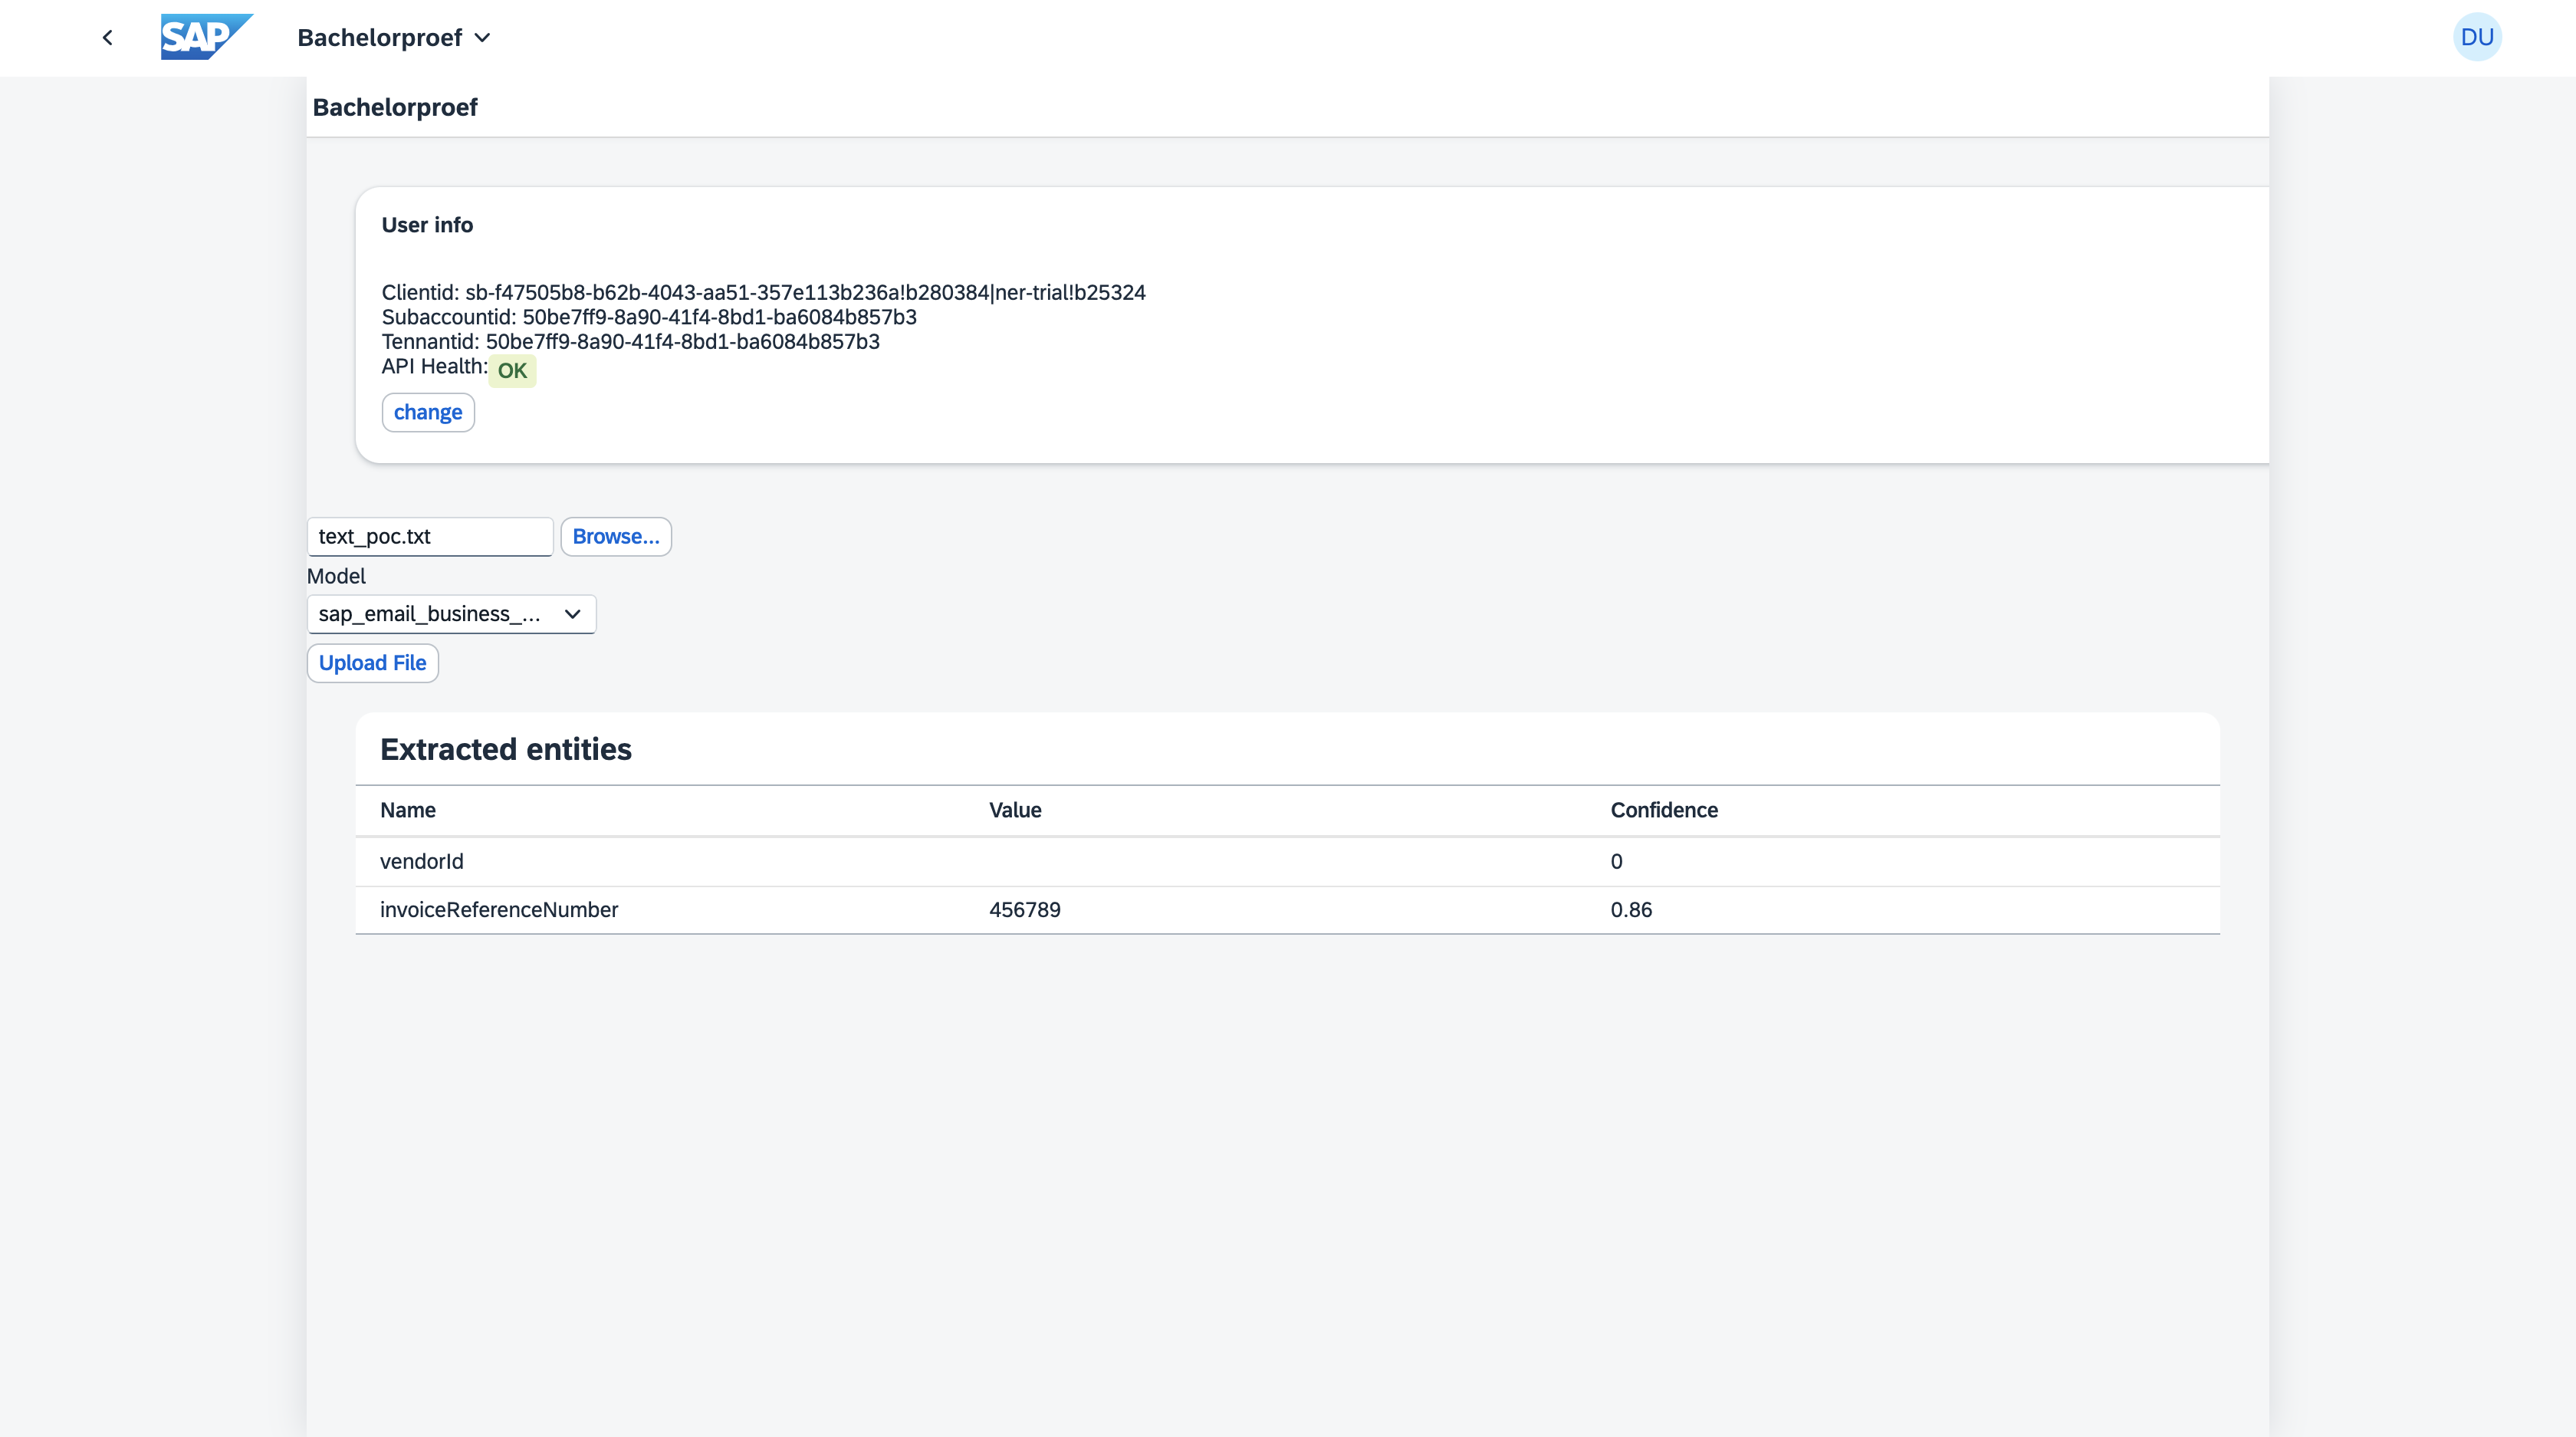
\includegraphics[width=0.8\textwidth]{./graphics/proof-of-concept.png}
    \caption{Proof of concept}
    \label{fig:proof-of-concept}
\end{figure}

\section{Benodigdheden}
Om de proof of concept uit te kunnen voeren wordt er verwacht dat er een aantal zaken reeds gekend of geïnstalleerd zijn. Deze zaken zijn de volgende:

\begin{itemize}
    \item \textbf{SAP BTP trail account:} Een trail account op de SAP Business Technology Platform (BTP) Cockpit, deze kan aangemaakt worden via: \url{https://account.hana.ondemand.com/}
    \item \textbf{Python:} Er wordt verwacht dat er een Python 3 installatie aanwezig is. Deze kan geïnstalleerd worden via: \url{https://www.python.org/downloads/}
    \item \textbf{Kennis van de gebruikte libraries:} Om de code in de proof of concept te kunnen begrijpen wordt er verwacht dat er een basiskennis van Flask en SAP Fiori aanwezig is.
    \item \textbf{Visual studio code: } Om gemakkelijk met SAP Fiori te kunnen werken wordt er aangeraden om Visual Studio Code te gebruiken. Dit omdat er een pakket met handige extensies beschikbaar is die het werken met SAP Fiori gemakkelijker maken, dit is te installeren via \url{https://marketplace.visualstudio.com/items?itemName=SAPSE.sap-ux-fiori-tools-extension-pack}. Een andere editor kan ook gebruikt worden, maar het opzetten van een project kan dan lastiger zijn.
\end{itemize}

\section{Github repository}
De volledige code van het proof-of-concept in dit onderzoek is online beschikbaar gesteld via GitHub. De repository bevat zowel de code van de api in de map \mintinline{bash}|api|, als de Fiori-applicatie in de map \mintinline{bash}|frontend|. De github repository is te vinden op \url{https://github.com/jamievschuerbeek/proof-of-concept-bachelorproef}.

\section{Opzetten van Business Entity Recognition in SAP BTP Cockpit}

Het SAP Business Technology Platform(BTP) is een online cloudplatform ontwikkeld door SAP waar er heel veel verschillende services door hen worden aangeboden en waar deze beheerd kunnen worden. De instances van deze services kunnen geheel aangepast worden aan de wensen en benodigdheden van de gebruiker doormiddel van configuratie en eigen ontwikkelingen.
Om de Business Entity Recognition service te gebruiken wordt er verwacht dat er in de SAP BTP Cockpit deze service wordt opgezet. Bij deze service kan er de configuratie aangepast worden om bijvoorbeeld eigen documenten toe te voegen die samen een dataset vormen. Deze dataset kan gebruikt worden om een eigen model te trainen.

\subsection{SAP BTP trail account}

Het SAP Business Technology Platform is opgedeeld in verschillende account: Een global account en één of meerdere subaccounts. De global account heeft toegang tot globale configuratie zoals het beheer van rollen en gebruikers die bepaalde subaccounts mogen zien en aanpassen. De subaccounts worden dan weer gebruikt om instanties van SAP-diensten op te draaien en beheren. Om op de SAP BTP Cockpit te geraken, dient er allereerst naar de homepagina van de \href{https://account.hana.ondemand.com/cockpit#/home/allaccounts}{BTP Cockpit} genavigeerd te worden. Hier kan verder via de knoppen op de pagina genavigeerd worden naar de hoofdpagina van het global trail account. Hier zijn een aantal pagina's te vinden die het mogelijk maken om verschillende zaken te beheren:
\begin{itemize}
    \item \textbf{Account explorer:} Hier kunnen de verschillende subaccounts beheerd worden.
    \item \textbf{Resource Providers:} Indien een gebruiker een eigen amazon aws of azure omgeving heeft, kan deze hier worden toegevoegd.
    \item \textbf{Boosters:} Boosters zijn tools die aangeboden worden door SAP die het gemakkelijk maken om een bepaalde service op te zetten. Meer informatie zal gegeven worden in sectie \ref{sec:ber-booster}.
    \item \textbf{System landscape:} Indien een gebruiker een SAP omgeving buiten het BTP heeft, kan deze hier worden toegevoegd.
    \item \textbf{Entitlements:} Hier kunnen de verschillende services die aangeboden worden door SAP worden beheerd.
    \item \textbf{Security:} Hier kunnen de verschillende gebruikers en rollen worden beheerd.
    \item \textbf{Usage: } Hier kan de gebruiker zien hoeveel van de verschillende services er gebruikt worden.
\end{itemize}

\subsection{Business Entity Recognition Booster}
\label{sec:ber-booster}
Om het aanmaken van de verschillende services een stuk gemakkelijker te maken, biedt SAP een aantal tools aan om deze automatisch op te zetten. Deze tools heten 'boosters' en ook voor de Business Entity Recognition service wordt er ook een booster aangeboden. Om de booster uit te voeren, dient er eerst naar de 'Boosters' pagina genavigeerd te worden op de SAP BTP Cockpit. Hier kan er gezocht worden naar de 'Set up account for Business Entity Recognition' booster en kan deze geactiveerd worden. 
\begin{figure}[H]
    \centering
    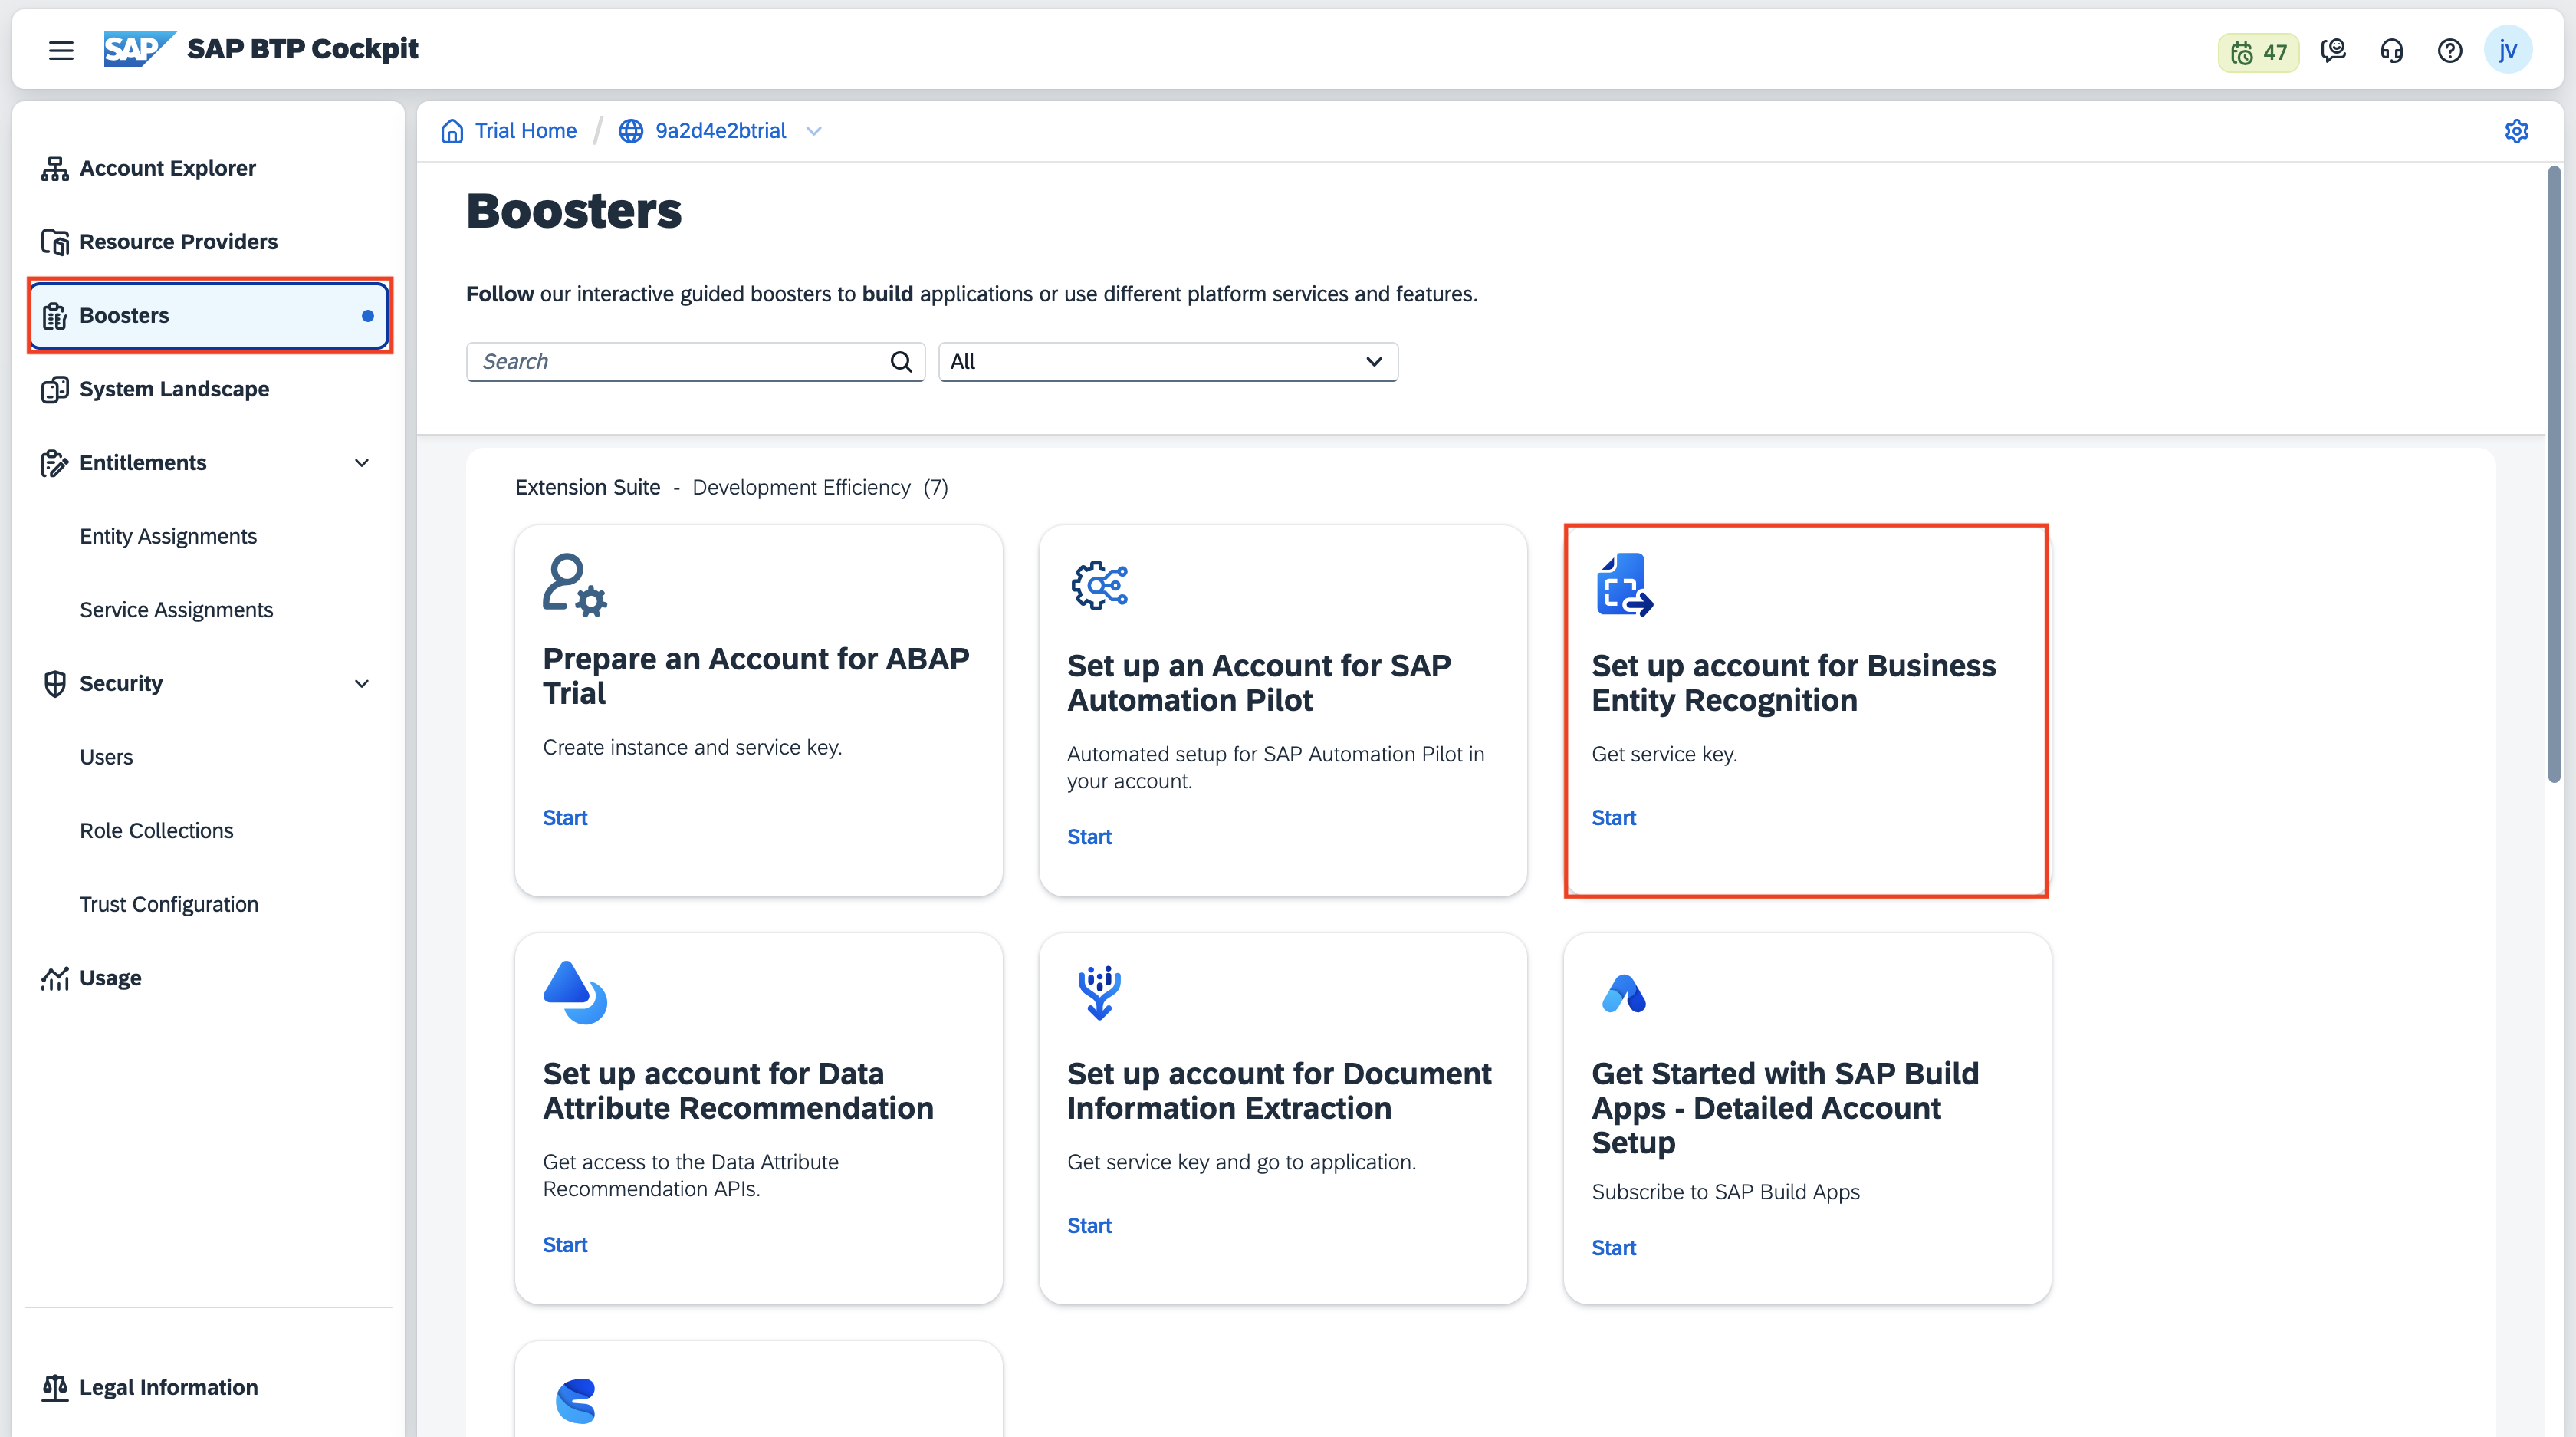
\includegraphics[width=0.8\textwidth]{./graphics/sap_btp_home_boosters.png}
    \caption{Business Entity Recognition booster}
    \label{fig:ber-booster}
\end{figure}

Na het activeren van de booster, zal er een scherm verschijnen waar de subaccount gekozen kan worden waar de service op kan draaien. Voor dit onderzoek is de standaard subaccount die aangemaakt wordt bij het aanmaken van een trail account voldoende. Verder kan er ook een space gemaakt worden waar de service in kan draaien, hiervoor is er de space 'bachelorproef' gemaakt. De booster zal dan een aantel zaken in het subaccount aanmaken en configureren, als dit allemaal gelukt is, zal er een melding verschijnen dat de booster succesvol is uitgevoerd zoals in figuur \ref{fig:booster-succes}. In deze melding staat er ook een link naar de service key die nodig is om de service aan te roepen, deze service key dient gedownload te worden en zal later in de applicatie gebruikt worden.

\begin{figure}[H]
    \centering
    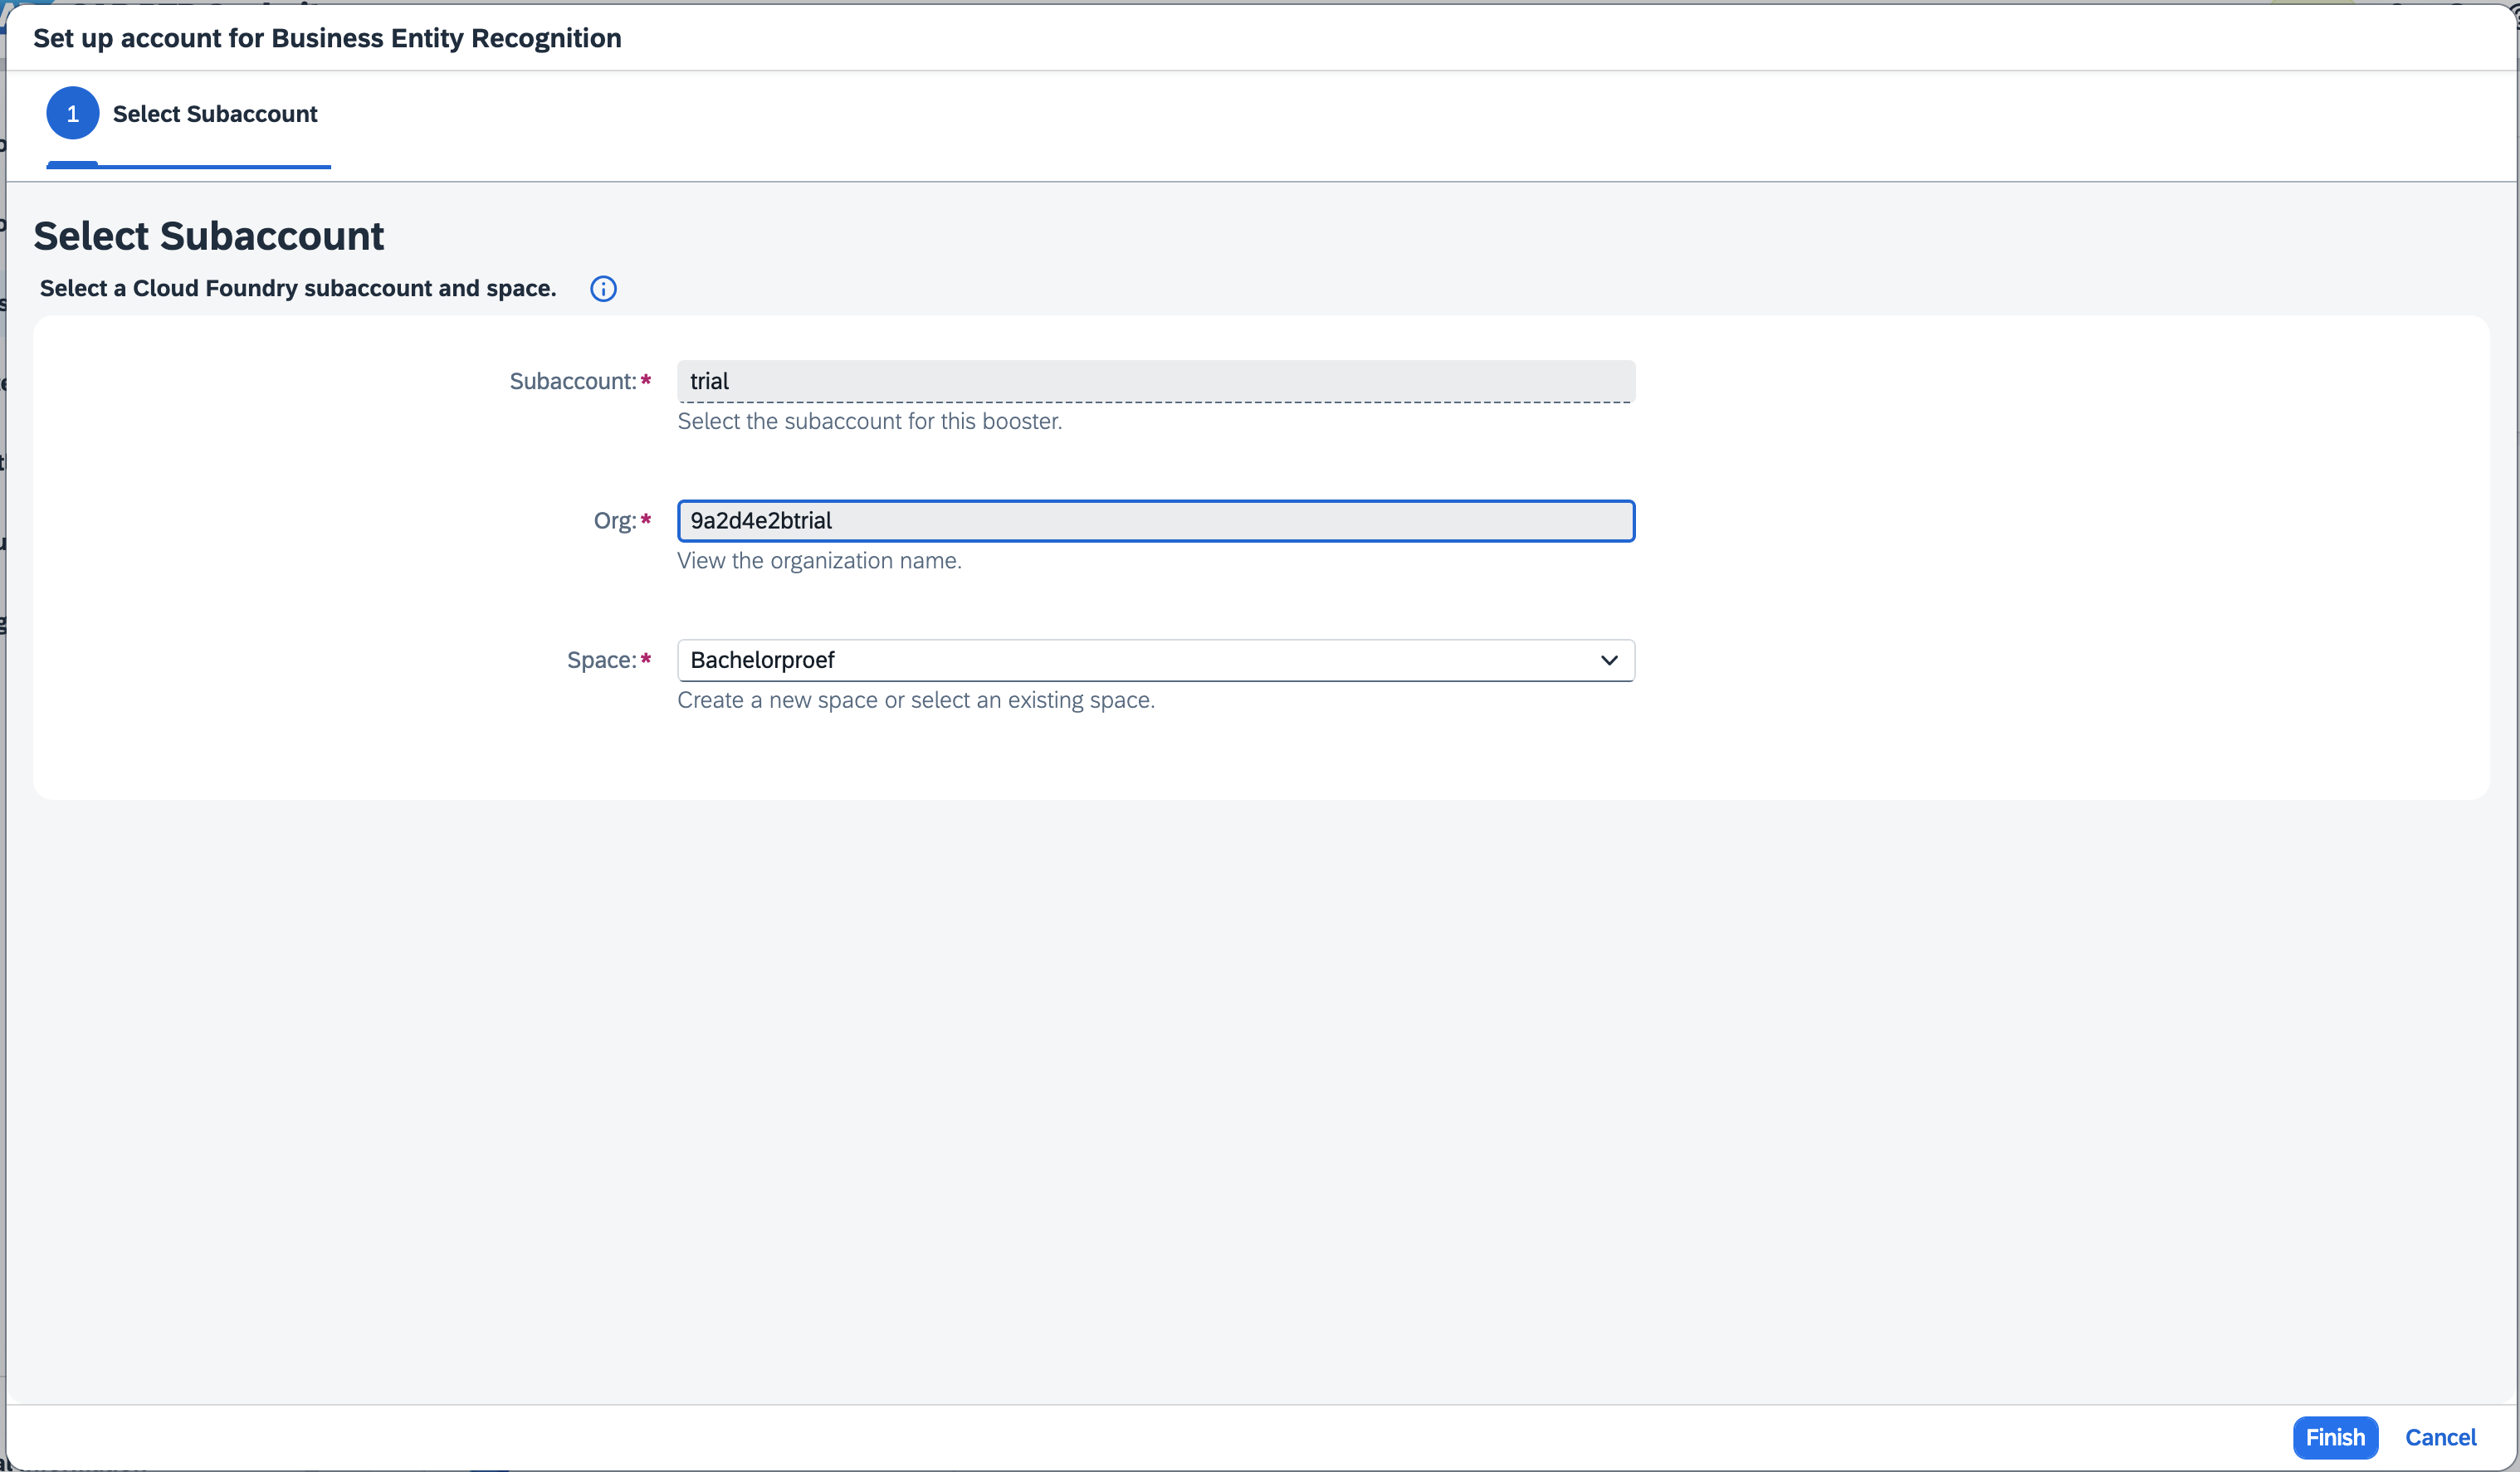
\includegraphics[width=0.8\textwidth]{./graphics/booster_subaccount.png}
    \caption{Booster subaccount selectie}
    \label{fig:booster-subaccount}
\end{figure}

\begin{figure}[H]
    \centering
    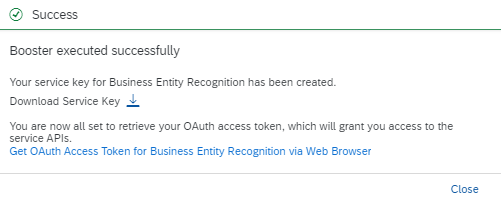
\includegraphics[width=0.8\textwidth]{./graphics/booster_succes.png}
    \caption{Booster succesvol uitgevoerd}
    \label{fig:booster-succes}
\end{figure}

\section{Python api}
\label{sec:python-api}

Om de Business Entity Recognition service te gebruiken heeft SAP een handige API beschikbaar gesteld die het mogelijk maakt om de service aan te roepen en te gebruiken. Hiervoor hebben ze ook een Python library gemaakt om dit gemakkelijk via code te gebruiken. Om een webapplicatie rond deze service te maken, zal er een eigen API gemaakt worden om zo meer controle te hebben over de data die er wordt opgevraagd en verstuurd.

Om de API in python te maken wordt er gebruik gemaakt van de Flask library. Flask is een library die het mogelijk maakt om snel verschillende soorten webapplicaties op te zetten. 

\subsection{Virtualenv en packages installeren}
Eerst wordt er doormiddel van virtualenv een nieuwe virtuele omgeving gemaakt. Er wordt een virtuele omgeving gemaakt omdat verschillende projecten verschillende dependencies kunnen hebben en deze op die manier niet met elkaar in conflict kunnen komen. Om een nieuwe virtuele omgeving te maken dient virtualenv geïnstalleerd met het volgende commando:
\begin{lstlisting}[language=bash]
    pip3 install virtualenv
\end{lstlisting}

Dan wordt er een map aangemaakt waarin de code zal komen, in dit voorbeeld wordt de map 'api' gemaakt waarin alle code van de api zal komen.
\begin{lstlisting}[language=bash]
    mkdir api
    cd api
\end{lstlisting}

Dan wordt de daadwerkelijke virtuele omgeving aangemaakt in de huidige map:

\begin{lstlisting}[language=bash]
    virtualenv .
\end{lstlisting}

Dit commando zorgt ervoor dat er virtuele omgeving in de map wordt gemaakt, het commando maakt ook een aantal mappen en bestanden aan die python nodig heeft om het project correct uit te voeren.
\begin{itemize}
    \item bin: Deze map bevat alle uitvoerbare bestanden die nodig zijn om de virtuele omgeving te activeren en te deactiveren.
    \item lib: Deze map bevat alle libraries die geïnstalleerd zijn in de virtuele omgeving.
    \item pyvenv.cfg: Dit bestand bevat de configuratie van de virtuele omgeving.
    \item .gitignore: Dit bestand bevat alle bestanden die niet mogen worden opgenomen in een git repository.
\end{itemize}

Uiteindelijk wordt de virtuele omgeving geactiveerd:
\begin{lstlisting}[language=bash]
    source bin/activate
\end{lstlisting}

Als de virtuele omgeving geactiveerd is, kan er begonnen worden met het installeren van de benodigde libraries. De libraries die geïnstalleerd moeten worden zijn de volgende:
\begin{itemize}
    \item Flask
    \item Flask-Cors
    \item sap-business-entity-recognition-client-library
\end{itemize}

Om deze libraries te installeren wordt er gebruik gemaakt van het volgende commando:
\begin{lstlisting}[language=bash]
    pip install Flask Flask-Cors sap-business-entity-recognition-client-library
\end{lstlisting}
Dit zal ervoor zorgen dat de libraries worden geïnstalleerd worden in de '/lib' map om later in de code te kunnen gebruiken.

Om de webserver te starten om de API te testen, wordt er gebruik gemaakt van het volgende commando:
\begin{lstlisting}[language=bash]
    flask run --reload
\end{lstlisting}

Dit commando zal de webserver starten en de API beschikbaar maken op \url{http://127.0.0.1:5000}. De optie '--reload' zorgt ervoor dat de webserver automatisch herstart wordt als er een aanpassing in de code wordt gemaakt. Dit maakt het gemakkelijker om de code te testen en aan te passen zonder dat de API constant manueel herstart moet worden.

\subsection{API code}

De code van de API wordt geplaatst in een bestand genaamd 'app.py'. De code bestaat uit een aantal methodes die de verschillende endpoints van de API vormen.
Om een API in flask te maken, worden eerst de verschillende dependencies geïmporteerd die in het project gebruikt zullen worden. Dan wordt er een instantie van de Flask klasse aangemaakt en wordt er een aantal configuraties ingesteld. De eerste endpoint die wordt aangemaakt is de '/health' endpoint. Deze endpoint is een eenvoudige methode die 'OK' antwoord om te controleren of de connectie met de API werkt.

\begin{listing}[H]
    \setminted{%
gobble=2,
}   
\begin{minted}{python3}
    from flask import Flask, jsonify, request
    from flask_cors import CORS, cross_origin
    from sap_ber_client import ber_api_client
    from time import sleep

    app = Flask(__name__)
    cors = CORS(app, origins="*")
    app.config['CORS_HEADERS'] = 'Content-Type'

    @app.route('/health')
    @cross_origin()
    def health():
        return jsonify("OK")
\end{minted}
\caption{Import van de dependencies en de '/health' endpoint in app.py}
\end{listing}

\paragraph{addAuth functie}
Om de Business Entity Recognition service te gebruiken wordt er een instantie van de ber\_api\_client klasse aangemaakt. Deze klasse heeft een aantal methodes die het mogelijk maken om de service te gebruiken. Om deze klasse te kunnen gebruiken, moet er eerst een aantal gegevens worden ingevuld die nodig zijn om de service te gebruiken. Hiervoor wordt er een methode 'addAuth' gebruikt die de gegevens van de gebruiker in elke vraag richting de API ophaalt en de instantie teruggeeft.
\begin{listing}[H]
    \setminted{%
gobble=2,
}   
\begin{minted}{python3}
    def addAuth(data):

    try:
        url = data['url']
        uaa_clientid = data['uaa']['clientid']
        uaa_clientsecret = data['uaa']['clientsecret']
        uaa_url = data['uaa']['url']
    
        return ber_api_client.BER_API_Client(url, uaa_clientid, 
                                    uaa_clientsecret, uaa_url)
    except:
        return None
\end{minted}
\caption{addAuth methode in app.py}
\end{listing}

\paragraph{API endpoints}

De api heeft een aantal endpoints die het mogelijk maken voor een gebruiker of applicatie om de service aan te roepen en een resultaat terug te krijgen. De '/models' route geeft een lijst van alle aanwezige modellen terug die gebruikt kunnen worden om een tekst te lezen. Op deze manier kan de gebruiker alle beschikbare modellen zien en kiezen welke hij wilt gebruiken. Deze modellen geven aan de BER-service wat context over wat voor tekst het precies is, wat betere resultaten op kan leveren.

De '/inference' route is de route die de tekst neemt samen met de naam van het model en die dit doorgeeft aan de BER-service. De service zal de tekst inlezen en de belanghebbende informatie eruit halen. De BER-service geeft een id terug van de 'job' die het document gekregen heeft, de methode wacht tot de service klaar is met het document te verwerken en haalt de informatie op aan de hand van dit id. De methode leest dan de resulaten in en geeft deze terug in een JSON formaat dat gemakkelijk te gebruiken is in de frontend applicatie.

\begin{listing}[H]
    \setminted{%
gobble=2,
}   
\begin{minted}{python3}
    @app.route('/models', methods=['POST'])
    @cross_origin()
    def getModels():
        ber_service = addAuth(request.get_json())

        if ber_service is None:
            return "No valid credentials provided", 400
    
        models = ber_service.get_trained_models()
        result = models.json()['data']['sapModels']['models']
        return jsonify({"items" : result})
\end{minted}
\caption{'/models' endpoint in app.py}
\end{listing}

\begin {listing}[H]
    \setminted{%
gobble=2,
}
\begin{minted}{python3}
    @app.route('/inference', methods=['POST'])
    @cross_origin()
    def inference():
        req_data = request.get_json()

        ber_service = addAuth(req_data['auth'])
        
        model_version = 1
        model_name = req_data['model']
        text = req_data['text']
        
        if ber_service is None:
            return "No valid credentials provided", 400
        

        inference_job = ber_service.post_inference_job(text,model_name, 
                                                        model_version)
        inference_jobid = inference_job.json()['data']['id']
        
        inference_job_result = ber_service.get_inference_job(inference_jobid)
        while inference_job_result.json()['data']['status'] == 'PENDING':
            inference_job_result = ber_service.get_inference_job(inference_jobid)
            sleep(1)

        response = inference_job_result.json()
        
        data = response['data']['result'][0]
        result = []
        for key in data.keys():
            if len(data[key]) == 0:
                merged = {"name": key, "value": '', "confidence": 0}
            else:
                merged = {"name": key} | data[key][0]
            result.append(merged)

        return jsonify({"items" : result})
\end{minted}
\caption{'/inference' endpoint in app.py}
\end{listing}

\paragraph{Note}
Om de code te laten werken, moet er een aanpassing gebeuren in de sap-business-entity-recognition-client-library. Deze gebruikt een verouderde versie van de requests library die ervoor zorgt dat de code niet werkt. Om dit op te lossen moet er in de \mintinline{bash}|/lib/sap_ber_client| map een aanpassing gebeuren aan de parameter in het \mintinline{bash}|http_request_retry.py| bestand. De parameter 'method\_whitelist' die wordt megegeven wordt aan het retry object moet worden aangepast naar 'allowed\_methods', zoals in codevoorbeeld \ref{code:allowed_methods}.
\begin{listing}[H]
    \setminted{
gobble=2,
}
\begin{minted}{python3}
    def retry_session(pool_maxsize=None, retries=3, backoff_factor=1,
    status_forcelist=(500, 502, 503, 504)):
    session = requests.Session()
    retry = Retry(total=retries,
                  read=retries,
                  status=retries,
                  connect=retries,
                  backoff_factor=backoff_factor,
                  status_forcelist=status_forcelist,
                  allowed_methods=['GET'],
                  raise_on_status=False)
    adapter = HTTPAdapter(max_retries=retry, pool_maxsize=pool_maxsize)
    session.mount('http://', adapter)
    session.mount('https://', adapter)
    return session
\end{minted}
\caption{Aanpassing in http\_request\_retry.py}
\label{code:allowed_methods}
\end{listing}

\section{Frontend applicatie}

In deze sectie wordt er toegelicht hoe de frontend applicatie is opgebouwd en hoe deze communiceert met de API die in sectie \ref{sec:python-api} is gemaakt. De frontend applicatie is een webapplicatie die gebruik maakt van SAP Fiori en is bedoeld om een gebruiksvriendelijke manier te bieden om de BER-service te gebruiken. 

\subsection{Opzetten van het Fiori project}

Om een Fiori-project aan te maken, biedt SAP een eenvoudige manier. In Visual Studio Code kan een nieuw project worden aangemaakt met behulp van de Fiori Application Generator. Deze generator biedt de mogelijkheid om een aantal zaken te configureren, zoals de naam, beschrijving en minimale versie van het project. Ook kan er een voorgebouwde template worden gekozen die een basis vormt voor het project en een externe data source zoals een SAP systeem. 

In deze proof of concept is er gekozen voor een basis template en zonder externe data source omdat deze later toegevoegd wordt in de code. De rest van de configuratie is de naam van de eerste view en het project zelf, zoals te zien is in figuur \ref{fig:fiori-generator}.

\begin{figure}[H]
    \centering
    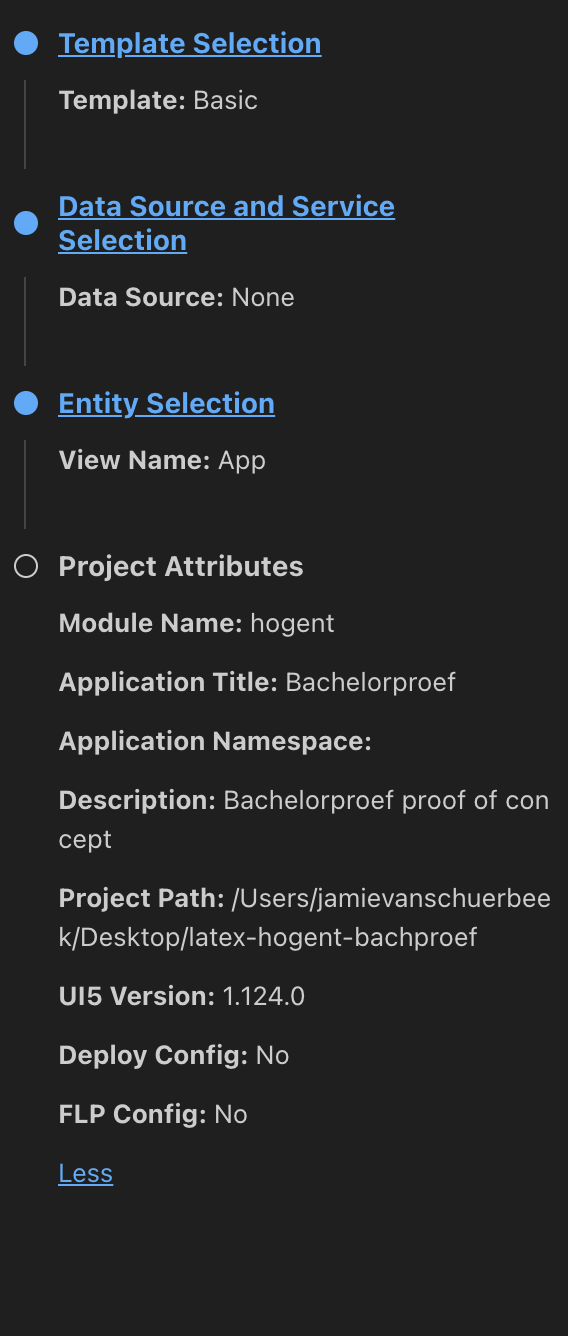
\includegraphics[scale=0.4]{./graphics/Fiori_config.png}
    \caption{Fiori application generator}
    \label{fig:fiori-generator}
\end{figure}

\subsection{Bestandenstructuur van de Fiori-applicatie}
De Fiori Application Generator maakt een aantal bestanden en mappen aan die het project correct laten werken. Deze structuur ziet er als volgt uit:

\begin{figure}[H]
    \centering
    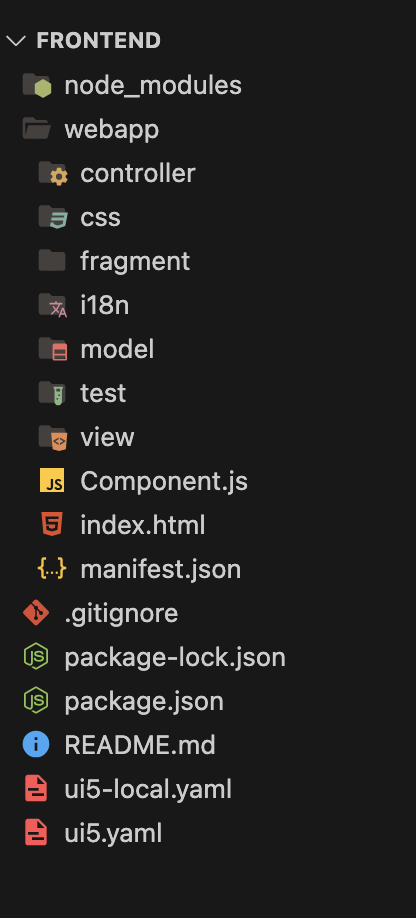
\includegraphics[scale=0.4]{./graphics/projectstructuur_fiori.png}
    \caption{Bestandenstructuur van het fiori project}
    \label{fig:fiori-generator}
\end{figure}

\begin{itemize}
    \item \textbf{node\_modules:} Bevat alle dependencies die aanwezig zijn in het project.
    \item \textbf{webapp:} Bevat alle code die de frontend van de applicatie vormt.
    \begin{itemize}
        \item \textbf{controller:} Bevat alle javascript controllers die de logica van de applicatie bedienen.
        \item \textbf{css:} Bevat alle css bestanden die de stijl van de app bepalen.
        \item \textbf{fragment: } Bevat alle fragments, dit zijn views die hergebruikt kunnen worden, zoals een dialoogvenster.
        \item \textbf{i18n:} Bevat alle vertalingen die de app ondersteunt.
        \item \textbf{model:} Bevat alle modellen die de app gebruikt, indien de app met een database zou werken.
        \item \textbf{test: } Bevat alle testen die geschreven zijn voor de app.
        \item \textbf{view:} Bevat alle views die de app heeft, deze views bepalen de structuur van de pagina.
        \item \textbf{Component.js:} Dit bestand is een component dat door ui5 wordt gemaakt die de app opstart.
        \item \textbf{index.html:} Dit bestand is de hoofdpagina van de app, hierin wordt de rest van de app in getoond.
        \item \textbf{manifest.json:} Dit bestand bevat alle configuratie van de app, zoals de naam, beschrijving en de versie.
    \end{itemize}
    \item \textbf{.gitignore:} Dit bestand bevat alle bestanden en mappen die niet mogen worden opgenomen in een git repository.
    \item \textbf{package.json en package-lock.json:} Deze bestanden bevatten alle info dependencies die nodig zijn om de app te laten werken.
    \item \textbf{ui5.yaml en ui5-local.yaml:} Deze bestanden bevatten alle ui5 configuratie.
\end{itemize}

\subsection{Eerste opstart}

Voordat de applicatie voor de eerste keer gestart kan worden, moeten eerst alle benodigde dependencies geïnstalleerd worden. Dit kan gedaan worden door het volgende commando uit te voeren.
\begin{lstlisting}[language=bash]
    npm install
\end{lstlisting}

Als dit commando uitgevoerd is, kan de applicatie voor het eerst gestart worden met het volgende commando:
\begin{lstlisting}[language=bash]
    npm start
\end{lstlisting}

Dit commando zal de ingebouwde webserver starten en de app openen in de webbrowser. 

\subsection{Code van de frontend: de views}

Als het project is opgezet, kan er begonnen worden met het effectief schrijven van de code die de frontend vormt. In dit onderzoek is er gekozen om alle functionaliteiten in één view te plaatsen. Dit zodat de gebruiker gemakkelijk alle functionaliteiten kan terugvinden en niet constant moet navigeren tussen verschillende paginas.

\paragraph{App view}

De app view is de eerst pagina die de gebruiker ziet als hij de app opent. In deze proof of concept is dit de enige pagina die de applicatie en deze heeft daarom heel veel elementen om alle functionaliteiten te kunnen gebruiken. 

Om een view te maken in SAP Fiori worden altijd een aantal namespaces gebruikt. Deze namespaces worden door SAP aangeboden om verschillende soorten voor gedefinieerde elementen te kunnen gebruiken voor verschillende doeleinden. In codevoorbeeld \ref{code:app-view} is te zien hoe de namespaces bovenaan de pagina worden geïmporteerd en hoe de basis van de pagina eruit ziet voor de rest van de componenten worden toegevoegd.

\begin{listing}[H]
    \setminted{%
gobble=2,
}
\begin{minted}{xml}
    <mvc:View controllerName="hogent.controller.App"
    xmlns:l="sap.ui.layout"
    xmlns:u="sap.ui.unified"
    xmlns:mvc="sap.ui.core.mvc" displayBlock="true"
    xmlns:core="sap.ui.core"
    xmlns:f="sap.f"
    xmlns:card="sap.f.cards"
    xmlns:tnt="sap.tnt"
    xmlns="sap.m">
    <Shell id="shell">
        <App id="app">
            <pages>
                <Page id="page" title="{i18n>title}">
                    <content>
                        <l:VerticalLayout>
                            <!-- REST VAN DE VIEW -->
                        </l:VerticalLayout>
                    </content>
                </Page>
            </pages>
        </App>
    </Shell>
</mvc:View>
\end{minted}
\caption{Namespaces importeren in app.view.xml}
\label{code:app-view}
\end{listing}

Als er een service key wordt geüpload, wordt er bovenaan de pagina een kaart getoond met alle gegevens van de huidige gebruiker. Ook wordt er een knop getoond die het mogelijk maakt om de huidige service key te veranderen indien een andere gebruiker de app wilt gebruiken. 
\begin{listing}[H]
    \setminted{%
gobble=2,
}
\begin{minted}{xml}
    <f:Card class="sapUiMediumMargin">
        <f:header>
            <card:Header title="User info"/>
        </f:header>
        <f:content>
            <VBox class="sapUiSmallMargin" justifyContent="SpaceBetween">
                <Text id="userClientId" text="Clientid: {auth>/uaa/clientid}"/>
                <Text id="userSubAccountId" text="Subaccountid: {auth>/uaa/subaccountid}"/>
                <Text id="userTennantId" text="Tennantid: {auth>/uaa/tenantid}"/>
                <HBox id="userApiHealth">
                    <Text text="API Health:"/>
                    <tnt:InfoLabel id="lblApiHealth" text="NOT AVAILABLE" colorScheme="2"/>
                </HBox>
                <Button text="change" press="openAuthDialog"/>
            </VBox>
        </f:content>
    </f:Card>
\end{minted}
\caption{User info kaart in app.view.xml}
\end{listing}

De belangrijkste functionaliteit van de app is het uploaden van een tekstbestand om daadwerkelijk een tekst te kunnen analyseren. Om dit te doen is er een fileuploader toegevoegd aan de pagina die het mogelijk maakt om een tekstbestand te kiezen op het apparaat van de gebruiker. Naast de fileuploader is er ook een menu toegevoegd die het mogelijk maakt om te kiezen uit een bestaand model om de context van de tekst te bepalen. De 'Upload file' knop zorgt dat in de controller het bestand naar de API wordt gestuurd zodat deze de tekst kan verwerken. Al deze zaken samen vormen de code die te zien is in codevoorbeeld \ref{code:fileuploader}.
\begin{listing}[H]
    \setminted{%
gobble=2,
}
\begin{minted}{xml}
    <u:FileUploader id="fileUploaderFS" name="fileUploaderFS" 
    uploadUrl="uploadFile" change="onFileChange" fileType="txt" 
    multiple="false" placeholder="Upload"/>
    <VBox alignContent="SpaceBetween">
        <Text text="Model"/>
        <ComboBox id="selectModel" items="{models>/items}">
            <core:Item key="{models>modelName}" text="{models>modelName}"/>
        </ComboBox>
    </VBox>
    <Button text="Upload File" press="handleUploadPress"/>
\end{minted}
\caption{Fileuploader en model selectie in app.view.xml}
\label{code:fileuploader}
\end{listing}

Als de API de tekst heeft verwerkt, wordt deze door de API teruggegeven in een JSON formaat. De controller zal deze data in een JSON model plaatsen zodat deze dat bereikbaar is in de view. De view zal dan de data in een tabel plaatsen zodat de gebruiker de resultaten kan zien.

\begin{listing}[H]
    \setminted{%
gobble=2,
}
\begin{minted}{xml}
    <Table headerText="Extracted entities" width="auto" 
    class="sapUiResponsiveMargin" items="{result>/items}">
            <columns>
                <Column>
                    <Text text="Name"/>
                </Column>
                <Column>
                    <Text text="Value"/>
                </Column>
                <Column>
                    <Text text="Confidence"/>
                </Column>
            </columns>
            <items>
                <ColumnListItem>
                    <cells>
                        <Text text="{result>name}"/>
                        <Text text="{result>value}"/>
                        <Text text="{result>confidence}"/>
                    </cells>
                </ColumnListItem>
            </items>
        </Table>
\end{minted}
\caption{Tabel met resultaten in app.view.xml}
\end{listing}

\paragraph{de UploadAuth fragment}
Om de service key toe te kunnen voegen, wordt er een dialoogvenster getoond die het mogelijk maakt om de service key te uploaden. Voor dit dialoogvenster wordt er een fragment view gemaakt waarin de structuur van het venster wordt bepaald.

Het dialoogvenster wordt getoond als de gebruiker de applicatie opent of als de gebruiker op de 'change' knop drukt. Als de gebruiker de service key heeft toegevoegd, wordt deze in de controller opgeslagen zodat deze kan worden gebruikt elke keer als de API wordt aangeroepen.

Bij het dialog-element wordt het \mintinline{xml}|afterClose| attribuut gebruikt om een methode aan te roepen in de controller als het dialoogvenster wordt gesloten. Dit zorgt ervoor dat de service key wordt opgeslagen in de controller en dat deze kan worden gebruikt in de rest van de applicatie.

\begin{listing}[H]
    \setminted{%
gobble=2,
}
\begin{minted}{xml}
    <core:FragmentDefinition xmlns="sap.m"
    xmlns:core="sap.ui.core"
    xmlns:l="sap.ui.layout"
    xmlns:u="sap.ui.unified"
    xmlns:f="sap.ui.layout.form">
    <Dialog id="dlgUploadAuth" title="Please upload your key.json" 
    afterClose="onAuthClose">
        <u:FileUploader id="authUploader" name="authUploader" 
        uploadUrl="uploadFile" change="onAuthFileChanged" multiple="false" 
        placeholder="Upload key.json" 
        typeMissmatch="typeMissmatch" fileSizeExceed="fileSizeExceed" />
    </Dialog>
</core:FragmentDefinition>
\end{minted}
\end{listing}

\subsection{Code van de frontend: de controller}

De controller zorgt ervoor dat er logica aan de view wordt toegevoegd. In de controller worden verschillende methodes gemaakt die uitgevoerd worden na een bepaalde actie in de view. 

\paragraph{De onInit en openAuthDialog methodes}

Een controller in een Fiori project begint eerst met het importeren van alle benodigde dependencies, deze worden als parameter doorgegeven aan de controller om ze daar te gebruiken. In de controller is er altijd eerst de \mintinline{javascript}|onInit| methode aanwezig die wordt aangeroepen als de pagina wordt geopende. In dit geval wordt hier de functie aangeroepen die het dialoogvenster opent om de service key te uploaden.

De \mintinline{javascript}|openAuthDialog| functie in de controller zorgt ervoor er geen bestaande dialoogvenster geopend is en daarna dat de fragment wordt ingeladen en getoond aan de gebruiker. 

De \mintinline{javascript}|onAuthClose| functie wordt uitgevoerd als het dialoogvenster wordt gesloten. Deze functie zorgt ervoor dat het venster correct wordt gesloten en dat de rest van de data in de applicatie wordt opgehaald.

\begin{listing}[H]
    \setminted{%
gobble=2,
}
\begin{minted}{javascript}
    sap.ui.define(
    [
        "sap/ui/core/mvc/Controller",
        "sap/ui/model/json/JSONModel",
        "sap/m/MessageToast",
    ],
    /**
     * @param {typeof sap.ui.core.mvc.Controller} Controller
     */
    function (Controller, JSONModel, MessageToast) {
        "use strict";

        const url = "http://127.0.0.1:5000";

        return Controller.extend("hogent.controller.App", {
        onInit: function () {
            this.openAuthDialog();
        },
        
        // REST VAN DE METHODES

        //Open auth dialog
        openAuthDialog: function () {
            if (this.byId("dlgUploadAuth")) {
                this.byId("dlgLogin").destroy();
                this.pDialog = null;
            }
            this.pDialog = this.loadFragment({
                name: "hogent.fragment.UploadAuth",
            });
            this.pDialog.then(function (oDialog) {
                oDialog.open();
            });
        },

            onAuthClose: function () {
            this.byId("dlgUploadAuth").destroy();
            this.pDialog = null;

            this.addUserInfo();
            this.fetchModels();
            },
        });
    });
\end{minted}
\caption{onInit en openAuthDialog methodes in App.controller.js}
\end{listing}


\paragraph{De addUserInfo en fetchModels methode}

De \mintinline{javascript}|addUserInfo| methode is een simple methode die de API aanroept en wacht op een antwoord. Als de API een antwoord teruggeeft wordt dit in de view geplaatst zodat de gebruiker kan zien dat de connectie met de API in orde is.

De \mintinline{javascript}|fetchModels| methode is een methode die de API aanroept om alle beschikbare modellen op te halen. Deze modellen worden dan in een JSON model geplaatst zodat deze in de view beschikbaar zijn om aan de gebruiker te laten zien.

\begin{listing}[H]
    \setminted{%
gobble=2,
}
\begin{minted}{javascript}
    //get all available models
    fetchModels: function () {
        fetch(url + "/models", {
          method: "POST",
          headers: {
            "Content-Type": "application/json",
          },
          body: JSON.stringify(this.getView().getModel("auth").getData()),
        })
          .then((response) => {
            return response.json();
          })
          .then((data) => {
            this.getView().setModel(new JSONModel(data), "models");
          });
      },

      //check if connection to API is OK
    addUserInfo: function () {
        var pUrl = url + "/health";

        fetch(pUrl, {
          method: "GET",
        })
          .then((response) => {
            return response.json();
          })
          .then((data) => {
            this.getView()
              .byId("lblApiHealth")
              .setText(data)
              .setColorScheme(data === "OK" ? 8 : 2);
          });
      },
\end{minted}
\caption{addUserInfo en fetchModels methodes in App.controller.js}
\end{listing}

\paragraph{De onFileChange methodes}

De \mintinline{javascript}|onFileChange| en \mintinline{javascript}|onAuhtFileChange| methodes zijn twee gelijkaardige methodes die worden aangeroepen als de gebruiker een bestand heeft gekozen in de fileuploader. Deze methodes zorgen ervoor dat het bestand in de controller via een JSON model wordt opgeslagen zodat deze kunnen gebruikt worden bij het verder oproepen van de API. Zij zullen zorgen dat wanneer de service key is geüpload, deze in de oproepen naar de API kunnen worden meegestuurd en dat het tekstbestand kan worden geüpload naar de API. 

\begin{listing}[H]
    \setminted{%
gobble=2,
}
\begin{minted}{javascript}
    //Hadle file change - read file content and store locally
    onFileChange: function (e) {
        var file = e.getParameter("files") && e.getParameter("files")[0];
        if (file && window.FileReader) {
          var reader = new FileReader();
          reader.onload = function (evn) {
            var strCSV = evn.target.result;
            console.log(strCSV);
            this.getView().setModel(
              new JSONModel({ text: strCSV }),
              "currentText"
            );
          }.bind(this);
          reader.readAsText(file);
        }
      },

      //Handle file change - change file on api
      onAuthFileChanged: function (e) {
        var file = e.getParameter("files") && e.getParameter("files")[0];
        if (file && window.FileReader) {
          var reader = new FileReader();
          reader.onload = function (evn) {
            var strCSV = evn.target.result;
            this.getView().setModel(new JSONModel(JSON.parse(strCSV)), "auth");

            this.byId("dlgUploadAuth").close();
          }.bind(this);
          reader.readAsText(file);
        }
      },
\end{minted}
\caption{onFileChange en onAuthFileChange methodes in App.controller.js}
\end{listing}

\paragraph{De handleUploadPress methode}

Één van de belangrijkste methodes in de controller is de \mintinline{javascript}|handleUploadPress| methode. Deze methode zorgt ervoor dat de tekst die de gebruiker wilt analyseren wordt geüpload naar de API. Deze methode wacht dan op het antwoord van de API en slaat deze op in de controller, zodat deze in de view in een overzichtelijke tabel kan worden getoond aan de gebruiker. 

\begin{listing}[H]
    \setminted{%
gobble=2,
}
\begin{minted}{javascript}
    handleUploadPress: function () {
        var pModel = this.getView().byId("selectModel").getSelectedItem();
        if (pModel === null) {
          MessageToast.show("No model selected");
          return;
        }

        fetch(url + "/inference", {
          method: "POST",
          headers: {
            "Content-Type": "application/json",
          },
          body: JSON.stringify({
            model: pModel.getKey(),
            auth: this.getView().getModel("auth").getData(),
            text: this.getView().getModel("currentText").getData().text,
          }),
        })
          .then((response) => {
            return response.json();
          })
          .then((data) => {
            console.log(data);
            this.getView().setModel(new JSONModel(data), "result");
          });
      }, 
\end{minted}
\caption{handleUploadPress methode in App.controller.js}
\end{listing}
